% issue2_gates.tex -- why ttauto reports spurious pseudo-Anosovs (issue #2)
% and how the Bestvina--Handel gate test fixes it.
%
% Build: latexmk -pdf issue2_gates.tex
\documentclass[12pt]{amsart}
\usepackage{amsmath,amssymb,amsthm}
\usepackage[margin=1in]{geometry}
\usepackage{booktabs}
\usepackage{array}
\usepackage{tikz}
\usetikzlibrary{arrows.meta,calc,positioning,decorations.markings,shapes.misc}
\usepackage{hyperref}
\hypersetup{colorlinks=true,linkcolor=blue!60!black,citecolor=blue!60!black,
  urlcolor=blue!60!black}

% --- macros borrowed from ttauto.tex, plus a few local ones ---
\newcommand{\anti}[1]{\bar{#1}}          % reversed edge
\newcommand{\code}[1]{\texttt{#1}}
\newcommand{\ho}{\varphi}                 % homeomorphism
\newcommand{\trk}{\tau}                   % train track
\newcommand{\Dg}{D}                       % derivative
\newcommand{\dirs}{\mathcal{E}}           % oriented edges (directions)
\newcommand{\gates}{\mathcal{G}}
\newcommand{\turns}{\mathcal{T}}
\newcommand{\per}{P}                      % peripheral loop
\newcommand{\lam}{\lambda}
\newcommand{\Trains}{\textsc{Trains}}
\newcommand{\ttauto}{\texttt{ttauto}}
\newcommand{\dir}[1]{\mathsf{#1}}         % a direction as a symbol
\newcommand{\set}[1]{\{#1\}}

\theoremstyle{plain}
\newtheorem{Theorem}{Theorem}[section]
\newtheorem{Proposition}[Theorem]{Proposition}
\newtheorem{Lemma}[Theorem]{Lemma}
\newtheorem{Corollary}[Theorem]{Corollary}
\theoremstyle{definition}
\newtheorem{Definition}[Theorem]{Definition}
\newtheorem{Remark}[Theorem]{Remark}
\newtheorem{Example}[Theorem]{Example}

\tikzset{
  main/.style={thick},
  side/.style={thick,blue!70!black},
  periph/.style={thick,red!70!black},
  image/.style={very thick,orange!90!black,-{Stealth[length=2.5mm]}},
  gate/.style={line width=2.5pt,gray!60,line cap=round},
  chord/.style={thick,dashed},
  vert/.style={circle,fill=black,inner sep=1.2pt},
  punct/.style={cross out,draw=black,thick,minimum size=4pt,inner sep=0pt},
  lbl/.style={font=\small},
}

\title[Spurious pseudo-Anosovs in \ttauto]{Spurious pseudo-Anosovs in
  \ttauto: the Bestvina--Handel gate condition}
\author{Claude (Fable 5.1, \texttt{claude-fable-5-1})}
\address{Written in Claude Code for Jean-Luc Thiffeault, in the
  \texttt{ttauto} repository, branch \texttt{iss002-spurious-pAs}}
\date{19 September 2026}

\begin{document}

\begin{abstract}
  The folding automaton in \ttauto\ certifies a closed folding path as
  pseudo-Anosov when its transition matrix on main edges is irreducible with
  dilatation above one.  This is necessary but not sufficient: the
  Bestvina--Handel theory also requires that, at every vertex of the
  associated graph map, the \emph{gates} be connected by
  \emph{infinitesimal edges}.  We recall the criterion, translate it into
  the data structures of \ttauto\ (multigons, prongs, sides), work out the
  known bad example in full, explain why the current word-level
  train-track map cannot express the test, and give a word-free formulation
  that composes along a folding path in linear time.  The implementation
  plan is in \code{ISSUE2\_IMPLEMENTATION\_PLAN.md}.
\end{abstract}

\maketitle
\tableofcontents

%======================================================================
\section{The symptom}
\label{sec:symptom}

Issue \#2 in the \ttauto\ tracker reads: ``very rarely, the algorithm finds
pA that aren't---they are reducible.''  The canonical case is the closed
path
\[
  29 \to 46 \to 43 \to 71 \to 88 \to 85 \to 29
\]
(1-based vertex numbers) in the main 90-vertex subautomaton of the stratum
$s = 3,3\,(2)$ on the disc with $n=6$ punctures (stratum~5 in the
interactive program's list).  Its composed transition matrix on the seven
main edges is
\begin{equation}
  \label{eq:TM}
  M =
  \begin{pmatrix}
    0&0&0&0&0&0&1\\
    1&1&1&0&0&0&0\\
    0&0&0&1&0&0&0\\
    1&2&0&0&0&0&0\\
    0&0&1&0&1&0&1\\
    0&0&1&0&2&0&0\\
    0&0&0&0&0&1&0
  \end{pmatrix},
  \qquad
  \chi_M(x) = x^7 - 2x^6 + x^5 - 4x^4 + 4x^3 - x^2 + 2x - 1,
\end{equation}
which is primitive with spectral radius $\lam = 2.01536$.  By the criterion
used in the search (irreducible matrix, $\lam > 1$; see
\code{descend\_graph} in \code{ttauto.hpp}) the path is recorded as
pseudo-Anosov.

The braid realising the path,
$\sigma_1\sigma_2\sigma_3\sigma_5^{-1}\sigma_4^{-1}\sigma_3^{-1}$ on six
strings, was worked out by hand (\code{notes\_badbraid.pdf}).  Fed to Toby
Hall's \Trains\ program~\cite{HallTrain} it gives ``Growth 2.01536, Entropy 0.700796,
Isotopy class is Reducible''.  Both the \Trains\ output and Hall's reply
of 1 May 2009 are kept in this directory.  His explanation:
\begin{quote}
  If you have an efficient graph map with an irreducible transition matrix,
  then the isotopy class is pA \emph{provided} that all the gates at each
  vertex are connected by infinitesimal edges (see Proposition 3.3.2 of
  BH).  In this example, the gates at vertices 2 and 6 are not all
  connected by infinitesimal edges.
\end{quote}
He also notes that the 4th puncture is fixed and that deleting the 4th
string gives the 5-braid $\sigma_1\sigma_2\sigma_4^{-1}\sigma_3^{-1}$, a
genuine pseudo-Anosov with the same growth $2.01536$.  So the dilatation is
right, the matrix is right, and the map is nevertheless reducible: the
reducing curve encloses the other five punctures and the fixed puncture sits
in the annulus between that curve and the boundary.

The rest of this note explains what the missing condition says
(\S\ref{sec:bh}), how it reads on \ttauto's data structures
(\S\ref{sec:dictionary}--\ref{sec:fold}), what it gives on the bad path
(\S\ref{sec:example}), how to compute it without ever writing down the
exponentially long image words (\S\ref{sec:wordfree}), and which labelling
conventions the implementation has to get right (\S\ref{sec:labels}).

%======================================================================
\section{Bestvina--Handel background}
\label{sec:bh}

The statements below are from Bestvina and Handel~\cite{Bestvina1995}
(a copy, \code{Bestvina1995.pdf}, is in this directory); the notation
follows Hall's exposition~\cite{HallBHchapter}.  Bestvina--Handel work with
a \emph{fibered surface} $F$ carrying the homeomorphism $\ho$, with a graph
$G$ (junctions collapsed to vertices, strips to edges) and an induced graph
map $g\colon G\to G$ sending vertices to vertices and edges to edge paths.
Write $\dirs(G)$ for the set of \emph{oriented edges}, or
\emph{directions}: each edge $e$ gives two directions $e$ and $\anti e$,
and the directions with initial vertex $v$ form the link of $v$, with a
natural cyclic order.

\begin{Definition}[derivative and gates, {\cite[\S1]{Bestvina1995}}]
  The \emph{derivative} $\Dg g\colon \dirs(G)\to\dirs(G)$ sends $E$ to the
  first edge crossed by the edge path $g(E)$.  Two directions are
  \emph{equivalent} if they have the same initial vertex and are
  identified by some power of $\Dg g$.  The equivalence classes are the
  \emph{gates}.  Distinct gates map to distinct gates, and each gate is a
  consecutive block in the cyclic order at its vertex.
\end{Definition}

An edge path $E_1E_2\cdots E_k$ passes through a vertex between $E_i$ and
$E_{i+1}$ by the two directions $\anti E_i$ (pointing back along $E_i$) and
$E_{i+1}$; we say it \emph{takes the turn} $(\anti E_i,E_{i+1})$.

\begin{Definition}[efficient, {\cite[Lemma 3.1.2]{Bestvina1995}}]
  The map $g$ is \emph{efficient} if every iterate $g^k$ sends each edge
  to an edge path that does not backtrack; equivalently, if $g(E)$ does not
  backtrack and determines distinct gates each time it passes through a
  vertex, for every edge $E$.
\end{Definition}

Bestvina and Handel remark that by the second form efficiency can be
checked in a predictable number of steps.  The last part of their
algorithm reduces a fibered surface until it is efficient with irreducible
transition matrix; \S3.3 of the paper then builds a train track from it.

\begin{Definition}[the train track $\trk$, {\cite[\S3.3]{Bestvina1995}}]
  Inside each junction $J$ draw a small circle $C_J$ and put a point
  $p(\gamma)$ on it for each gate $\gamma$ at $J$, in the cyclic order.  The
  \emph{real edges} of $\trk$ are the edges of $G$, attached at the
  appropriate $p(\gamma)$.  Join $p(\gamma_1)$ and $p(\gamma_2)$ by an
  \emph{infinitesimal edge} if and only if for some edge $e$ of $G$ and
  some $m>0$ the edge path $g^m(e)$ enters $J$ through $\gamma_1$ and exits
  through $\gamma_2$.  The map $g$ induces a map on $\trk$: each real edge
  $e$ goes to $g(e)$ with the appropriate infinitesimal edge inserted
  between consecutive edges, and each infinitesimal edge goes to another
  infinitesimal edge.
\end{Definition}

\begin{Proposition}[{\cite[Prop.~3.3.2]{Bestvina1995}}]
  \label{prop:bh}
  If some component of $S\setminus\trk$ is not a disc, or equivalently if
  the union of the infinitesimal edges inside some $C_J$ fails to connect
  all the gates at $J$, then $\ho$ is isotopic to a reducible
  homeomorphism.
\end{Proposition}
\begin{proof}[Proof (from the paper)]
  The regular neighbourhood $N$ of $\trk$ has an essential non-peripheral
  boundary component; after an isotopy $\ho(N)=N$, which is a reduction.
\end{proof}

Conversely, if every component of $S\setminus\trk$ is a disc (one
containing the puncture, the others ``infinitesimal polygons'' inside the
$C_J$), then $\trk$ is a Thurston train track, and \S3.4 of the paper
constructs the Markov partition and the invariant measured foliations:
$\ho$ is pseudo-Anosov with dilatation $\lam(M_H)$
(\cite[Thm.~3.1.4]{Bestvina1995}, and \cite[Thm.~4.1.4]{Bestvina1995} for
several punctures).  This is the direction Hall quotes: efficient,
irreducible, gates connected, hence pA.  Together the two directions say
that for an efficient irreducible map the matrix decides nothing and the
gate graphs decide everything.

The paper also pins down what the infinitesimal edges can look like when
$\ho$ is pseudo-Anosov, which gives the implementation a cheap sanity
check.

\begin{Proposition}[{\cite[Props.~3.3.3--3.3.4]{Bestvina1995}}]
  \label{prop:shape}
  Suppose $g$ is efficient and irreducible with $\lam>1$ and every
  component of $S\setminus\trk$ is a disc.  Then every junction has at
  least two gates, and at a junction with $k$ gates the infinitesimal edges
  form either the single edge joining the two gates ($k=2$), or a
  $k$-gon joining adjacent gates, or a $k$-gon with exactly one side
  missing.
\end{Proposition}

Finally, several punctures (\cite[\S4]{Bestvina1995}) are handled by
requiring $G$ to contain a $g$-invariant \emph{peripheral subgraph} $P$
whose components are circles around the punctures, on which $g$ is a
homeomorphism.  With $\text{pre-}P$ the edges eventually mapped into $P$
and $H$ the rest, the transition matrix is block triangular and the growth
rate is that of $M_H$; the paper remarks that the edges of
$P\cup\text{pre-}P$ ``can be thought of as infinitesimal'' and are given
length zero.  Gates and efficiency are defined exactly as before.  Their
irreducibility condition (I2) says that if two distinct directions have
the same derivative then that common derivative lies in $H$; in
particular a peripheral direction is always a gate by itself.  In
\ttauto\ the peripheral subgraph is the set of loops of the punctured
monogons, and the main edges are $H$.

%======================================================================
\section{Dictionary: Bestvina--Handel versus \ttauto}
\label{sec:dictionary}

\ttauto\ never writes down a graph map.  It manipulates train tracks
directly (\cite[\S2--3]{Lanneau2011}): a track is a list of
\emph{multigons}, each a $k$-gon with $k$ \emph{prongs}; at each prong a
linearly ordered list of \emph{main edges} is attached, and two consecutive
edges at the same prong form a \emph{cusp}.  A punctured monogon ($k=1$)
encloses a puncture.  The sides of the multigons are the infinitesimal
edges of the paper's \S2.  Figure~\ref{fig:blowup} shows that this is the
blown-up picture of \S\ref{sec:bh} with the roles fixed as follows.

\begin{table}[h]
  \centering
  \begin{tabular}{@{}ll@{}}
    \toprule
    Bestvina--Handel & \ttauto \\
    \midrule
    vertex $v$ & an unpunctured multigon, taken as a whole; \\
               & or \emph{one prong} of a punctured multigon \\
    direction at $v$ & a signed main edge with tail at $v$; \\
                     & at a punctured multigon also the two directions
                       $\per,\anti\per$ of the loop \\
    gate at $v$ & a prong (a priori); refined by $\Dg^k$-coincidence \\
    infinitesimal edge & a side of an \emph{unpunctured} multigon that
                         some iterate traverses \\
    peripheral edge & a side of a \emph{punctured} multigon (the loop of a
                      monogon) \\
    main-edge matrix $M_H$ & the transition matrix on the $n$ main edges \\
    turn taken by $g^k(e)$ & consecutive main letters $x\,S\,y$ of an image
                             word, joining $\anti x$ to $y$ \\
    \bottomrule
  \end{tabular}
  \caption{The dictionary.  A side of a punctured multigon is a real
    (peripheral) edge of $G$, so its two ends are two different vertices
    when $k\ge2$ and the same vertex when $k=1$.}
  \label{tab:dictionary}
\end{table}

\begin{figure}[t]
  \centering
  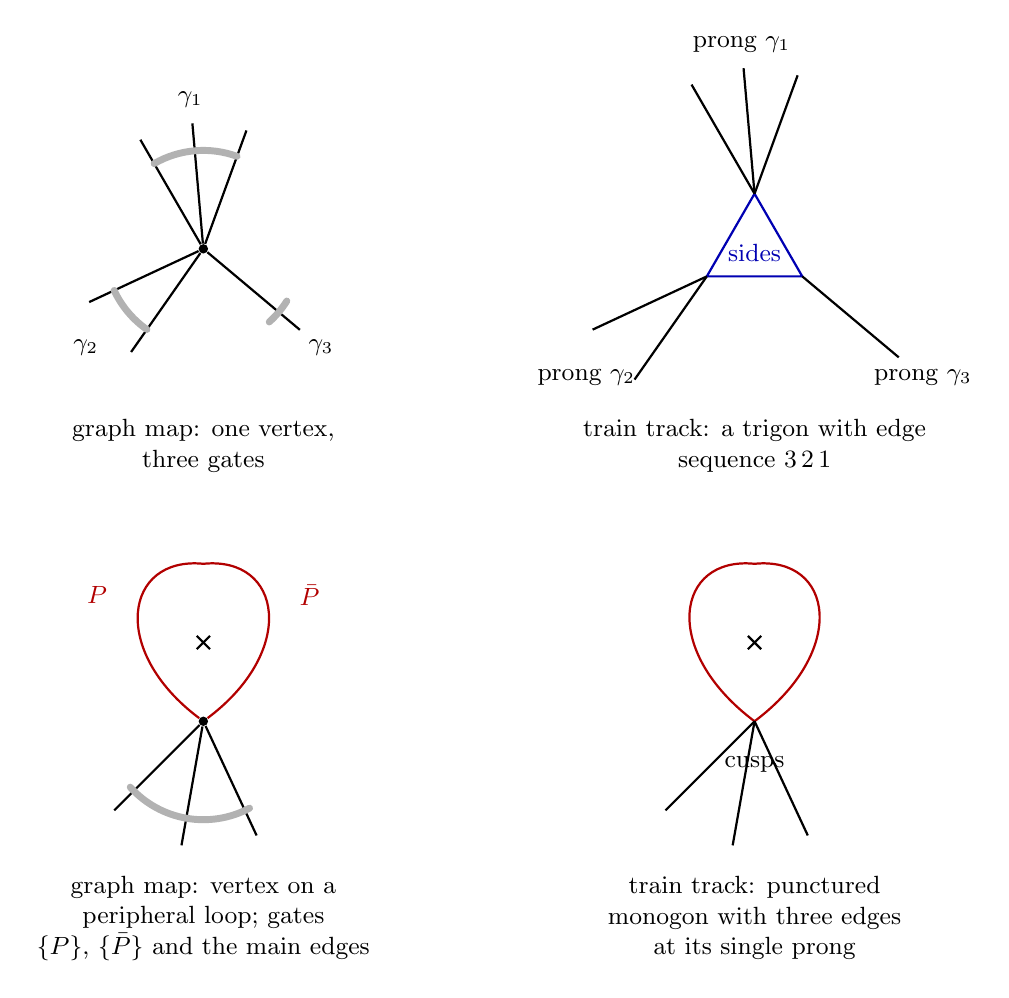
\begin{tikzpicture}[scale=1.0]
    % --- top left: graph vertex with three gates ---
    \begin{scope}
      \node[vert] (v) at (0,0) {};
      \foreach \a in {70,95,120} \draw[main] (v) -- (\a:1.6);
      \foreach \a in {205,235} \draw[main] (v) -- (\a:1.6);
      \draw[main] (v) -- (320:1.6);
      \draw[gate] (70:1.25) arc (70:120:1.25);
      \draw[gate] (205:1.25) arc (205:235:1.25);
      \draw[gate] (312:1.25) arc (312:328:1.25);
      \node[lbl] at (95:1.9) {$\gamma_1$};
      \node[lbl] at (220:1.95) {$\gamma_2$};
      \node[lbl] at (320:1.95) {$\gamma_3$};
      \node[lbl,align=center] at (0,-2.5) {graph map: one vertex,\\ three gates};
    \end{scope}
    % --- top right: blown-up triangle (ttauto trigon) ---
    \begin{scope}[xshift=7cm]
      \coordinate (A) at (90:0.7);
      \coordinate (B) at (210:0.7);
      \coordinate (C) at (330:0.7);
      \draw[side] (A) -- (B) -- (C) -- cycle;
      \foreach \a in {70,95,120} \draw[main] (A) .. controls ($(A)+(\a:0.8)$) .. ($(A)+(\a:1.6)$);
      \foreach \a in {205,235} \draw[main] (B) .. controls ($(B)+(\a:0.8)$) .. ($(B)+(\a:1.6)$);
      \draw[main] (C) .. controls ($(C)+(320:0.8)$) .. ($(C)+(320:1.6)$);
      \node[lbl] at ($(A)+(95:1.9)$) {prong $\gamma_1$};
      \node[lbl] at ($(B)+(220:2.0)$) {prong $\gamma_2$};
      \node[lbl] at ($(C)+(320:2.0)$) {prong $\gamma_3$};
      \node[lbl,blue!70!black] at (0,-0.05) {sides};
      \node[lbl,align=center] at (0,-2.5) {train track: a trigon with edge\\ sequence $3\,2\,1$};
    \end{scope}
    % --- bottom left: puncture with peripheral loop ---
    \begin{scope}[yshift=-6cm]
      \node[vert] (v) at (0,0) {};
      \node[punct] at (0,1.0) {};
      \draw[periph] (v) .. controls (-1.2,0.9) and (-1.0,2.1) .. (0,2.0)
                        .. controls (1.0,2.1) and (1.2,0.9) .. (v);
      \node[lbl,red!70!black] at (-1.35,1.6) {$\per$};
      \node[lbl,red!70!black] at (1.35,1.6) {$\anti\per$};
      \foreach \a in {225,260,295} \draw[main] (v) -- (\a:1.6);
      \draw[gate] (222:1.25) arc (222:298:1.25);
      \node[lbl,align=center] at (0,-2.5) {graph map: vertex on a\\ peripheral loop; gates\\ $\set{\per}$, $\set{\anti\per}$ and the main edges};
    \end{scope}
    % --- bottom right: ttauto punctured monogon ---
    \begin{scope}[xshift=7cm,yshift=-6cm]
      \coordinate (c) at (0,0);
      \node[punct] at (0,1.0) {};
      \draw[periph] (c) .. controls (-1.2,0.9) and (-1.0,2.1) .. (0,2.0)
                        .. controls (1.0,2.1) and (1.2,0.9) .. (c);
      \foreach \a in {225,260,295} \draw[main] (c) .. controls ($(c)+(\a:0.9)$) .. (\a:1.6);
      \node[lbl] at (0,-0.55) {cusps};
      \node[lbl,align=center] at (0,-2.5) {train track: punctured\\ monogon with three edges\\ at its single prong};
    \end{scope}
  \end{tikzpicture}
  \caption{The blow-up.  Top: a graph-map vertex with three gates is the
    same object as a \ttauto\ trigon whose corners are the prongs and whose
    sides are infinitesimal edges.  Bottom: a puncture; the peripheral loop
    $\per$ is a real edge of $G$, and in \ttauto\ it is the side of the
    punctured monogon.  The main edges at the single prong are pairwise
    separated by cusps.}
  \label{fig:blowup}
\end{figure}

Three consequences of the dictionary are used below.

\begin{Lemma}
  \label{lem:refine}
  Gates refine prongs: two directions at different prongs of the same
  multigon are never equivalent.
\end{Lemma}
\begin{proof}
  A fold never changes the number of prongs of any multigon; it detaches one
  end of an edge from a prong and re-attaches it at a prong of another
  multigon.  So along a folding path the prongs of the start track are
  mapped bijectively to the prongs of the end track, and $\Dg^k(E)$ has its
  tail at the image prong of the tail of $E$.  Directions at different
  prongs have images at different prongs, hence never coincide.
\end{proof}

\begin{Lemma}
  \label{lem:alternate}
  Every image word of a main edge under a composed fold map alternates
  main letters and side letters, begins and ends with a main letter, and
  never contains two consecutive side letters.
\end{Lemma}
\begin{proof}
  A single fold maps every main edge either to a single main letter or to
  $x\,S\,y$ with $x,y$ main and $S$ a side (\S\ref{sec:fold}); sides map to
  single sides.  Substituting such words into such words preserves the
  pattern.
\end{proof}

\begin{Corollary}
  \label{cor:efficient}
  Every realised turn is between two different prongs, hence between two
  different gates: the graph maps produced by folding paths are efficient
  automatically.
\end{Corollary}
\begin{proof}
  By Lemma~\ref{lem:alternate} a turn is always $x\,S\,y$ with $S$ a side
  from one prong to the next; so $\anti x$ and $y$ are at different prongs
  of that multigon, and by Lemma~\ref{lem:refine} in different gates.
\end{proof}

So in \ttauto\ the gate test is exactly: at every unpunctured multigon, do
the sides realised by iterates connect all the gates; and at every prong of
a punctured multigon, do the realised turns connect the main-edge gates to
the two peripheral directions $\per,\anti\per$ and to each other?

The shape constraint of Proposition~\ref{prop:shape} collapses this test
considerably at punctures.

\begin{Corollary}
  \label{cor:puncture}
  Let $v$ be a prong of a punctured multigon, with incoming peripheral side
  $\per_{\mathrm{in}}$, outgoing peripheral side $\per_{\mathrm{out}}$,
  and main gates $\mu_1,\dots,\mu_r$ in cyclic order between them.  The
  only infinitesimal edges that can be realised at $v$ are
  $\anti\per_{\mathrm{in}}$--$\mu_1$ and $\mu_r$--$\per_{\mathrm{out}}$.
  Hence the gate graph at $v$ is connected if and only if $r=1$ (the prong
  is a single gate) and both of these turns are taken by some iterate.
\end{Corollary}
\begin{proof}
  A turn joining two main gates at the same prong would be a turn inside
  a prong, excluded by Lemma~\ref{lem:alternate}.  A turn joining
  $\anti\per_{\mathrm{in}}$ to $\per_{\mathrm{out}}$ would come from two
  consecutive peripheral letters in the image of a main edge, also excluded
  by Lemma~\ref{lem:alternate}; images of peripheral edges are single
  letters and take no turns.  So at most the two named edges exist, and
  they connect all $r+2$ gates only when $r=1$.
\end{proof}

At a punctured monogon ($\per_{\mathrm{in}}=\per_{\mathrm{out}}=\per$)
this says: reducibility at a puncture shows up either as a \emph{refined
prong} (two main edges at the prong whose cusp is never folded, the bad
vertex of \S\ref{sec:example}) or as a loop that is never traversed in
one of its two senses.  When the test passes, the infinitesimal edges at
the prong are the path $\anti\per$--$\mu$--$\per$, the triangle with one
side missing of Proposition~\ref{prop:shape}(3).

\begin{Corollary}
  \label{cor:unpunctured}
  At an unpunctured $k$-gon with connected gate graph, at most one prong
  is refined, and then into exactly two gates.
\end{Corollary}
\begin{proof}
  Two gates in the same prong are adjacent in the cyclic order and cannot
  be joined (Lemma~\ref{lem:alternate}), so each refined prong costs one
  missing side of the polygon on the gates; Proposition~\ref{prop:shape}
  allows at most one missing side.
\end{proof}

The general union-find over gates and realised turns handles all of this
uniformly and is what the implementation does; the two corollaries are
what make the criterion easy to reason about, and they give sharp
assertions for the tests.

%======================================================================
\section{What one fold does to the map}
\label{sec:fold}

\begin{figure}[t]
  \centering
  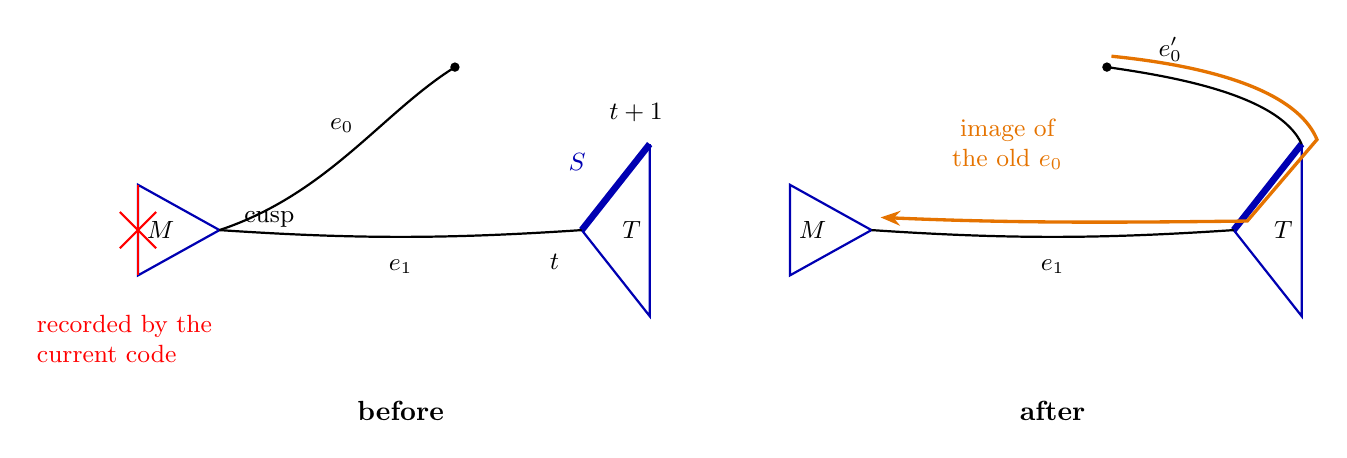
\begin{tikzpicture}[scale=1.15]
    % ---------------- before ----------------
    \begin{scope}
      % cusp multigon M (triangle) with right corner at (0,0)
      \coordinate (m0) at (0,0);
      \coordinate (m1) at (-0.9,0.5);
      \coordinate (m2) at (-0.9,-0.5);
      \draw[side] (m0) -- (m1) -- (m2) -- cycle;
      \node[lbl] at (-0.65,0) {$M$};
      % target multigon T with corner t_pr at (4,0), t2_pr at (4.75,0.9)
      \coordinate (t0) at (4,0);
      \coordinate (t1) at (4.75,0.95);
      \coordinate (t2) at (4.75,-0.95);
      \draw[side] (t0) -- (t2) -- (t1);
      \draw[side,line width=2.4pt] (t0) -- (t1);
      \node[lbl] at (4.55,0) {$T$};
      \node[lbl] at (3.7,-0.35) {$t$};
      \node[lbl] at (4.6,1.3) {$t+1$};
      \node[lbl,blue!70!black] at (3.95,0.75) {$S$};
      % e1 from M to T at prong t
      \draw[main] (m0) .. controls (1.5,-0.1) and (2.5,-0.1) .. (t0);
      \node[lbl] at (2,-0.4) {$e_1$};
      % e0 from M upward to far end
      \draw[main] (m0) .. controls (1.2,0.4) and (1.8,1.3) .. (2.6,1.8);
      \node[vert] at (2.6,1.8) {};
      \node[lbl] at (1.35,1.15) {$e_0$};
      \node[lbl] at (0.55,0.12) {cusp};
      % the side the code records today
      \draw[red,thick] (-0.9,0.5) -- (-0.9,-0.5);
      \draw[red,thick] (-1.1,0.2) -- (-0.7,-0.2);
      \draw[red,thick] (-1.1,-0.2) -- (-0.7,0.2);
      \node[lbl,red,align=left] at (-1.05,-1.2) {recorded by the\\ current code};
      \node at (2,-2.0) {\textbf{before}};
    \end{scope}
    % ---------------- after ----------------
    \begin{scope}[xshift=7.2cm]
      \coordinate (m0) at (0,0);
      \coordinate (m1) at (-0.9,0.5);
      \coordinate (m2) at (-0.9,-0.5);
      \draw[side] (m0) -- (m1) -- (m2) -- cycle;
      \node[lbl] at (-0.65,0) {$M$};
      \coordinate (t0) at (4,0);
      \coordinate (t1) at (4.75,0.95);
      \coordinate (t2) at (4.75,-0.95);
      \draw[side] (t0) -- (t2) -- (t1);
      \draw[side,line width=2.4pt] (t0) -- (t1);
      \node[lbl] at (4.55,0) {$T$};
      % e1 unchanged
      \draw[main] (m0) .. controls (1.5,-0.1) and (2.5,-0.1) .. (t0);
      \node[lbl] at (2,-0.4) {$e_1$};
      % e0' from far end to T at prong t+1
      \draw[main] (2.6,1.8) .. controls (3.3,1.7) and (4.5,1.5) .. (t1);
      \node[vert] at (2.6,1.8) {};
      \node[lbl] at (3.3,2.0) {$e_0'$};
      % image path of old e0: e0' then S then e1 (offset slightly)
      \draw[image] (2.65,1.92) .. controls (3.35,1.85) and (4.65,1.65) .. (4.92,1.0)
        -- (4.15,0.1) .. controls (2.5,0.08) and (1.5,0.08) .. (0.1,0.14);
      \node[lbl,orange!90!black,align=center] at (1.5,0.95) {image of\\ the old $e_0$};
      \node at (2,-2.0) {\textbf{after}};
    \end{scope}
  \end{tikzpicture}
  \caption{Folding $e_0$ onto $e_1$ at a cusp of the multigon $M$ (fold
    direction $+1$).  The end of $e_0$ at $M$ slides along $e_1$ to the
    target multigon $T$, arriving at prong $t$, and then along the side $S$
    of $T$ to the next prong $t+1$, where it re-attaches.  The image of the
    old edge $e_0$ (oriented from its far end towards $M$) is the path
    $e_0'\,S\,e_1$.  The side traversed is a side of the \emph{target}
    multigon, not of the cusp multigon whose side the current
    \code{fold\_infinitesimal\_generator} reports.}
  \label{fig:fold}
\end{figure}

Consider a fold at a cusp of multigon $M$ between consecutive edges $e_0$
and $e_1$ at the same prong, folding $e_0$ onto $e_1$
(Figure~\ref{fig:fold}).  In \code{traintrack::fold(multigon\&,p,c,dir)}:
$e_1$ has its other end at the target multigon $T$, prong $t$; the fold is
legal only if $e_1$ is the last (for direction $+1$) or first (for $-1$)
edge at that prong; then the end of $e_0$ at $M$ is detached and inserted
as the first (or last) edge at prong $t' = t \pm 1 \pmod k$ of $T$, where
$k$ is the number of prongs of $T$.  For a punctured monogon target
($k=1$) we have $t'=t$ and the edge goes once around the puncture.  Finally
\code{normalise()} is called.

The train-track map records what happened to each old edge as a path in
the new track:
\begin{itemize}
  \item every edge other than $e_0$ maps to itself (relabelled);
  \item the old $e_0$, oriented from its far end towards the cusp, maps to
    $e_0'\; S\; e_1$, where $S$ is the side of $T$ traversed from $t'$ to
    $t$; with the opposite orientation of $e_0$ the image is
    $\anti{e_1}\,\anti S\,\anti{e_0'}$.
\end{itemize}
The side letter is therefore determined by three things: the \emph{target}
multigon $T$, the prong pair $(t,t')$, and the orientation of $e_0$.  The
weights (transition matrix) see only the abelianisation of this: $e_0
\mapsto e_0' + e_1$.

\subsection*{What \code{fold\_traintrack\_map} does today}
The template in \code{include/traintracks/map.hpp} gets the permutation
part and the pair $(e_0',e_1)$ from the transition matrix (correct), then
\begin{enumerate}
  \item takes the side letter from
    \code{traintrack::fold\_infinitesimal\_generator(f,n)}, which resolves
    the \emph{cusp} location and returns the side of $M$ at the cusp prong.
    In all six folds of the bad cycle this is a different multigon from
    $T$ (Table~\ref{tab:folds});
  \item labels sides by position in the multigon vector \code{mgv} and lets
    every side map to itself, although \code{normalise()} reorders
    multigons and rotates prongs after every fold, and although the
    position of a multigon in \code{mgv} is not even canonical
    (structurally identical monogons sort in arbitrary order);
  \item chooses the word order $\{e_0',S,e_1\}$ versus $\{e_1,S,e_0'\}$
    from the parity of the fold index and always writes $S$ positively,
    with no reference to an orientation of $e_0$.
\end{enumerate}
Item 3 means the words are not edge paths.  Composing the stored one-step
words along the bad cycle and checking that consecutive letters share an
endpoint fails for every main edge (for instance the letter $-1$ is claimed
to start at monogon~1, which edge~1 does not touch).  Only the
abelianisation was ever tested, in \code{check\_fold\_map\_main\_transition},
and that function is compiled out in release builds.  Items~1 and~2 mean
that even the abelianised side data is wrong.  None of this affects the
transition matrices or anything the automaton reports; it only means the
word-level map produced for issue~\#3 cannot yet be used for gates.

%======================================================================
\section{The bad path worked out}
\label{sec:example}

Everything in this section was computed by \code{gates\_check.cpp}, which
rebuilds the one-step maps with correct sides and orientations from the
fold geometry, composes them exactly as the automaton composes matrices,
and runs the gate test.  It checks that the composite abelianises to $M$ of
\eqref{eq:TM} and that three iterates of every image word are continuous
edge paths.

\subsection{The train track at vertex 29}
Multigons: five punctured monogons $0,\dots,4$ with one edge each, one
punctured monogon $5$ with three edges, and two unpunctured trigons $6,7$
with one edge per prong.  Main edges, with the orientation used in the
tables (tail $\to$ head; $(m,p)$ means multigon $m$, prong $p$):
\[
  \begin{array}{ll@{\qquad}ll}
    1\colon (0,0)\to(5,0) & 2\colon (5,0)\to(6,0) & 3\colon (1,0)\to(6,1) & 4\colon (2,0)\to(6,2)\\
    5\colon (5,0)\to(7,0) & 6\colon (3,0)\to(7,1) & 7\colon (4,0)\to(7,2) &
  \end{array}
\]
Sides are numbered after the main edges: $8,\dots,13$ are the loops
$\per_0,\dots,\per_5$ of the six monogons; $14,15,16$ are the sides of
trigon~6 from prong $0\to1$, $1\to2$, $2\to0$; $17,18,19$ those of
trigon~7.  At monogon~5 the three edges sit at the single prong in the
slot order $1,2,5$.

\subsection{The six folds}

\begin{table}[h]
  \centering
  \small
  \begin{tabular}{@{}cccccccc@{}}
    \toprule
    step & vertices & $f$ & moved & onto & cusp at & target, side & code's side \\
    \midrule
    0 & $29\to46$ & 1 & 2 & 1 & monogon 5 (3 edges) & monogon 0, loop & monogon 5 \\
    1 & $46\to43$ & 0 & 4 & 3 & monogon 5 (2 edges) & trigon 6, $0\to1$ & monogon 5 \\
    2 & $43\to71$ & 3 & 5 & 4 & trigon 7 (2 edges)  & monogon 5, loop & trigon 7 \\
    3 & $71\to88$ & 2 & 5 & 1 & monogon 5 (3 edges) & monogon 0, loop & monogon 5 \\
    4 & $88\to85$ & 1 & 4 & 3 & monogon 5 (2 edges) & trigon 6, $0\to2$ & monogon 5 \\
    5 & $85\to29$ & 2 & 7 & 4 & trigon 7 (2 edges)  & monogon 5, loop & trigon 7 \\
    \bottomrule
  \end{tabular}
  \caption{The folds along the bad cycle.  Edge and multigon numbers are
    those of the stored track at the source vertex of each step (they are
    relabelled by \code{normalise()} at every step).  The last two columns
    contrast the side actually traversed with the one the current code
    records.}
  \label{tab:folds}
\end{table}

The corresponding one-step words (in the labels of the target vertex,
sides numbered as above) are
\begin{align*}
  \text{step 0:}\quad & 1\mapsto\anti4,\; 2\mapsto 4\,\anti{13}\,3,\; 3\mapsto1,\; 4\mapsto2,\; 5\mapsto5,\; 6\mapsto6,\; 7\mapsto7;\\
  \text{step 1:}\quad & 1\mapsto5,\; 2\mapsto6,\; 3\mapsto7,\; 4\mapsto 4\,\anti{19}\,\anti7,\; 5\mapsto3,\; 6\mapsto1,\; 7\mapsto2;\\
  \text{step 2:}\quad & 1\mapsto6,\; 2\mapsto7,\; 3\mapsto5,\; 4\mapsto2,\; 5\mapsto 1\,13\,2,\; 6\mapsto3,\; 7\mapsto4;\\
  \text{step 3:}\quad & 1\mapsto\anti4,\; 2\mapsto5,\; 3\mapsto6,\; 4\mapsto7,\; 5\mapsto 4\,13\,3,\; 6\mapsto1,\; 7\mapsto2;\\
  \text{step 4:}\quad & 1\mapsto6,\; 2\mapsto7,\; 3\mapsto5,\; 4\mapsto 4\,17\,\anti5,\; 5\mapsto3,\; 6\mapsto1,\; 7\mapsto2;\\
  \text{step 5:}\quad & 1\mapsto3,\; 2\mapsto4,\; 3\mapsto2,\; 4\mapsto5,\; 5\mapsto6,\; 6\mapsto7,\; 7\mapsto 1\,\anti{13}\,5.
\end{align*}
Every step also permutes the twelve sides; for example step~0 sends the
loops $8,9,10,11,12,13$ of monogons $0,\dots,5$ to $12,8,9,10,11,13$,
because the monogon that received the folded edge has become a 2-edge
monogon and \code{normalise()} moves it.

\subsection{The composed map}
Composing (each word substituted into the next) gives, in the labels of
vertex 29,
\begin{equation}
  \label{eq:AM}
  \begin{aligned}
    1 &\mapsto 4\;16\;\anti2, &
    2 &\mapsto 2\;\anti{16}\;\anti4\;\anti{10}\;4, &
    3 &\mapsto 6\;\anti{17}\;\anti5\;13\;2, &
    4 &\mapsto 3,\\
    5 &\mapsto 5\;17\;\anti6\;11\;6, &
    6 &\mapsto 7, &
    7 &\mapsto 1\;\anti{13}\;5, &&
  \end{aligned}
\end{equation}
and on sides $8\mapsto10$, $9\mapsto11$, $10\mapsto9$, $11\mapsto12$,
$12\mapsto8$, $13\mapsto13$, $14\mapsto16$, $15\mapsto14$, $16\mapsto15$,
$17\mapsto18$, $18\mapsto19$, $19\mapsto17$.  Continuity can be checked by
eye: in $1\mapsto 4\,16\,\anti2$, edge~4 ends at $(6,2)$, side~16 runs from
prong~2 to prong~0 of trigon~6, and $\anti2$ starts at the head of~2, which
is $(6,0)$.  Counting main letters reproduces~\eqref{eq:TM}.  The loop of
the 3-edge monogon, $13$, is fixed: that monogon is the fixed puncture.

\subsection{Derivative, gates, joins}
The derivative on main directions is read off from the first letters of
\eqref{eq:AM} and of the inverse words:
\[
  \begin{array}{r@{\;\mapsto\;}l@{\qquad}r@{\;\mapsto\;}l}
    1 & 4 & \anti1 & 2 \\
    2 & 2 & \anti2 & \anti4 \\
    3 & 6 & \anti3 & \anti2 \\
    4 & 3 & \anti4 & \anti3 \\
    5 & 5 & \anti5 & \anti6 \\
    6 & 7 & \anti6 & \anti7 \\
    7 & 1 & \anti7 & \anti5
  \end{array}
\]
and on peripheral directions it is the side permutation above.  The turns
taken by the one-step images in \eqref{eq:AM}, written as unordered pairs
of directions, are
\[
  (\anti{13},\anti1),\ (\anti{13},2),\ (\anti{11},6),\ (\anti{10},4),\
  (\anti6,\anti5),\ (\anti4,\anti2),\ (4,10),\ (5,13),\ (6,11),
\]
and closing this set under $(E,E')\mapsto(\Dg E,\Dg E')$ adds nothing
new here.  Table~\ref{tab:gates} lists, for each Bestvina--Handel vertex,
the directions, the gates and the joins.

\begin{table}[h]
  \centering
  \small
  \begin{tabular}{@{}llll@{}}
    \toprule
    vertex & gates & joins & connected \\
    \midrule
    monogon 0 (puncture)  & $\set{\anti8},\set{1},\set{8}$ & $\anti8\!\sim\!1,\ 1\!\sim\!8$ & yes \\
    monogon 1 (puncture)  & $\set{\anti9},\set{3},\set{9}$ & $\anti9\!\sim\!3,\ 3\!\sim\!9$ & yes \\
    monogon 2 (puncture)  & $\set{\anti{10}},\set{4},\set{10}$ & $\anti{10}\!\sim\!4,\ 4\!\sim\!10$ & yes \\
    monogon 3 (puncture)  & $\set{\anti{11}},\set{6},\set{11}$ & $\anti{11}\!\sim\!6,\ 6\!\sim\!11$ & yes \\
    monogon 4 (puncture)  & $\set{\anti{12}},\set{7},\set{12}$ & $\anti{12}\!\sim\!7,\ 7\!\sim\!12$ & yes \\
    monogon 5 (puncture, fixed) & $\set{\anti{13}},\set{\anti1,2},\set{5},\set{13}$
       & $\anti{13}\!\sim\!\anti1,\ \anti{13}\!\sim\!2,\ 5\!\sim\!13$ & \textbf{no} (2 components) \\
    trigon 6 & $\set{\anti2},\set{\anti3},\set{\anti4}$ & all three pairs & yes \\
    trigon 7 & $\set{\anti5},\set{\anti6},\set{\anti7}$ & all three pairs & yes \\
    \bottomrule
  \end{tabular}
  \caption{Gate analysis of the bad path at vertex 29.  At the five 1-edge
    monogons the loop is traversed in both senses by some image, joining
    $\per$ and $\anti\per$ to the main gate.  At the trigons the gates are
    the prongs and all three sides are realised.  At the fixed 3-edge
    monogon the main prong splits into two gates and the loop joins each
    of them to only one of its own ends.}
  \label{tab:gates}
\end{table}

\subsection{The bad vertex}
At monogon~5 the directions are $\anti1$ (edge~1 ends there), $2$, $5$ and
the two loop directions $13=\per_5$ and $\anti{13}$.  Since $\Dg(\anti1) =
\Dg(2) = 2$, the directions $\anti1$ and $2$ are one gate; $5$ is another,
because its $\Dg$-orbit $5\to5$ never meets the orbit $2\to2$.  So the
single prong carries \emph{two} gates: the cusp between edges~2 and~5 is
never folded along the cycle.  The joins come from the subwords
$1\,\anti{13}\,5$ (in the image of~7) and $\anti5\,13\,2$ (in the image
of~3): the loop is traversed only from the $\set{\anti1,2}$ side to the
$\set5$ side, never the other way.  Hence the gate graph has the two
components $\set{\anti{13},\anti1,2}$ and $\set{13,5}$
(Figure~\ref{fig:badvertex}, left): two disjoint infinitesimal edges on
four gates, so by Proposition~\ref{prop:bh} the map is reducible.  The
healthy vertices of Table~\ref{tab:gates} all show one of the shapes
allowed by Proposition~\ref{prop:shape}: at the 1-edge monogons the
infinitesimal edges form the path $\anti\per$--main--$\per$, a triangle
with the side $\per\anti\per$ missing, and at the trigons a full
triangle.

\begin{figure}[t]
  \centering
  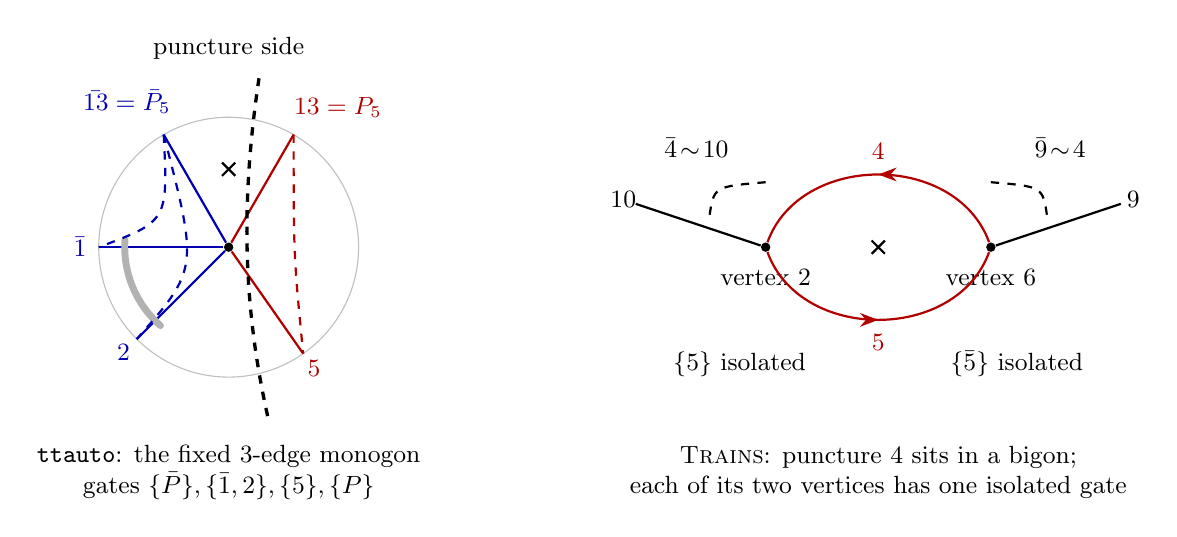
\begin{tikzpicture}[scale=1.1]
    % ------------- left: ttauto monogon 5 -------------
    \begin{scope}
      \node[vert] (v) at (0,0) {};
      \draw[gray!50] (0,0) circle (1.5);
      % directions: Pbar 120, 1bar 180, 2 225, 5 305, P 60
      \draw[periph,blue!70!black] (v) -- (120:1.5);
      \node[lbl,blue!70!black] at (125:2.05) {$\anti{13}=\anti\per_5$};
      \draw[periph,red!70!black]  (v) -- (60:1.5);
      \node[lbl,red!70!black] at (52:2.05) {$13=\per_5$};
      \draw[main,blue!70!black] (v) -- (180:1.5) node[pos=1.15,lbl] {$\anti1$};
      \draw[main,blue!70!black] (v) -- (225:1.5) node[pos=1.15,lbl] {$2$};
      \draw[main,red!70!black]  (v) -- (305:1.5) node[pos=1.15,lbl] {$5$};
      \node[punct] at (90:0.9) {};
      \node[lbl] at (90:2.3) {puncture side};
      % gate arc around {1bar,2}
      \draw[gate] (176:1.2) arc (176:229:1.2);
      % joins as chords
      \draw[chord,blue!70!black] (120:1.5) .. controls (-0.7,0.3) .. (180:1.5);
      \draw[chord,blue!70!black] (120:1.5) .. controls (-0.35,-0.25) .. (225:1.5);
      \draw[chord,red!70!black]  (60:1.5)  .. controls (0.75,-0.1)  .. (305:1.5);
      % local separating curve between the two components
      \draw[very thick,dashed,black] (0.45,-1.95) .. controls (0.15,-0.6) and (0.15,0.6) .. (0.35,1.95);
      \node[lbl,align=center] at (0,-2.6) {\ttauto: the fixed 3-edge monogon\\
        gates $\set{\anti\per},\set{\anti1,2},\set5,\set\per$};
    \end{scope}
    % ------------- right: Trains bigon -------------
    \begin{scope}[xshift=7.5cm]
      \node[vert] (a) at (-1.3,0) {};
      \node[vert] (b) at (1.3,0) {};
      \node[lbl] at (-1.3,-0.35) {vertex 2};
      \node[lbl] at (1.3,-0.35) {vertex 6};
      \node[punct] at (0,0) {};
      % peripheral edges 4 (top, 6->2) and 5 (bottom, 2->6)
      \draw[periph,postaction={decorate},decoration={markings,mark=at position 0.5 with {\arrow{Stealth}}}]
        (b) .. controls (0.9,1.1) and (-0.9,1.1) .. (a);
      \draw[periph,postaction={decorate},decoration={markings,mark=at position 0.5 with {\arrow{Stealth}}}]
        (a) .. controls (-0.9,-1.1) and (0.9,-1.1) .. (b);
      \node[lbl,red!70!black] at (0,1.1) {$4$};
      \node[lbl,red!70!black] at (0,-1.1) {$5$};
      % main edges 10 at vertex 2 (leaving left), 9 at vertex 6 (arriving from right)
      \draw[main] (a) -- (-2.8,0.5) node[lbl,pos=1.1] {$10$};
      \draw[main] (b) -- (2.8,0.5) node[lbl,pos=1.1] {$9$};
      % joins
      \draw[chord] (-1.3,0.75) .. controls (-1.9,0.7) .. (-1.95,0.35);
      \node[lbl,align=left] at (-2.1,1.15) {$\anti4\!\sim\!10$};
      \draw[chord] (1.3,0.75) .. controls (1.9,0.7) .. (1.95,0.35);
      \node[lbl,align=left] at (2.1,1.15) {$\anti9\!\sim\!4$};
      \node[lbl] at (-1.6,-1.35) {$\set5$ isolated};
      \node[lbl] at (1.6,-1.35) {$\set{\anti5}$ isolated};
      \node[lbl,align=center] at (0,-2.6) {\Trains: puncture 4 sits in a bigon;\\
        each of its two vertices has one isolated gate};
    \end{scope}
  \end{tikzpicture}
  \caption{The reducibility seen at the fixed puncture.  Left: the
    directions at \ttauto's monogon~5 on a small circle, the gate
    $\set{\anti1,2}$ marked by a grey arc, joins as dashed chords.  The two
    colours are the two components of the gate graph; the black dashed arc
    separates them locally, and its global continuation is the reducing
    curve around the other five punctures.  Right: the same phenomenon in
    Hall's train track, where puncture~4 is enclosed by two peripheral
    edges $4,5$ meeting at vertices 2 and 6; images run $9\to4\to10$ and
    never use edge~5.}
  \label{fig:badvertex}
\end{figure}

\subsection{Comparison with Trains}
Hall's program found a different invariant train track for the same
braid: puncture~4 sits in a punctured \emph{bigon} whose two peripheral
edges $4$ and $5$ meet at vertices~2 and~6, with main edge~10 attached at
vertex~2 and main edge~9 at vertex~6 (Figure~\ref{fig:badvertex}, right).
Its output reports the gates $\set{10},\set{5},\set{\anti4}$ at vertex~2,
joined only by $\anti4\sim10$, and $\set{4},\set{\anti5},\set{\anti9}$ at
vertex~6, joined only by $\anti9\sim4$: images arrive along~9, go half way
round the puncture along~4, and leave along~10, never touching~5.  This is
the same fact as our two components, expressed on a track where the
puncture's vertex has been split in two.  Since the two tracks are
different, comparing them vertex by vertex (as the reproducer
\code{tests/test\_issue2\_bad\_path.cpp} tried to do) is meaningless; only
the verdict is comparable.  The reproducer's own gate pipeline also failed
for a structural reason: it took each $(\text{multigon},\text{prong})$ pair
as a vertex and the infinitesimal letters as directions at it, then linked
the two ends of every side.  In that model every monogon is disconnected
whatever the dynamics, which is what it reported.

\subsection{Positive controls}
The same program run on four closed paths that the automaton reports as
pseudo-Anosov in the same subautomaton, the cycles (0-based)
$\{28,45,42,45,28\}$ ($\lam=2.453$), $\{2,37,39,19,22,20,12,2\}$
($\lam=2.081$), $\{4,84,28,45,28,80,4\}$ ($\lam=2.453$) and
$\{21,42,45,28,45,42,21\}$ ($\lam=3.254$), finds every gate graph
connected, with the shapes of Proposition~\ref{prop:shape} at every
vertex.  A fifth control, $\{1,18,65,18,56,57,57,1\}$, could not be
analysed by the scratch program because of its own branch bookkeeping; the
library implementation described in \S\ref{sec:plan} accepts it.

\subsection{Census over all strata}
\label{sec:census}
Once the test was in the library, it was run inside the search on the
main subautomaton of every stratum for $n=3,\dots,7$, with the path
lengths of the strata scan (\code{examples/ttauto\_scan\_strata.sh}).
The bad path is not the only spurious pseudo-Anosov, but every rejection
has the same shape.

\begin{table}[h]
  \centering
  \small
  \begin{tabular}{@{}cllcl@{}}
    \toprule
    $n$ & stratum & rejected $\lam$ (paths) & vertex & interpretation \\
    \midrule
    4 & $(2)$ & $2.61803$ (3) & 3-edge monogon & $\sigma_1\sigma_2^{-1}$ on 3 strings plus an idle puncture; \\
      &       &               &                & characteristic polynomial $(x-1)(x^2-3x+1)$; a genuine \\
      &       &               &                & class with the same dilatation is still accepted \\
    6 & $4\,(2)$ & $1.61803$ & unpunctured 4-gon & matrix irreducible but not primitive \\
      &          &           &                   & (eigenvalues $\pm\varphi$) \\
    6 & $4\,(2)$ & $1.93185$ & unpunctured 4-gon & likewise irreducible but not primitive \\
      &          &           &                   & (polynomial in $x^2$, eigenvalues $\pm1.93185$) \\
    6 & $4\,(2)$ & $2.15372$ & 3-edge monogon & the $n=5$, $4\,(1)$ minimum plus an idle puncture \\
    6 & $3\,3\,(2)$ & $2.01536$ (3) & 3-edge monogon & the bad path of this note \\
    6 & $3\,3\,(2)$ & $2.54205$ (8) & 3-edge monogon & two length-8 extensions of the bad cycle \\
      &             &               &                & (one repeats its last two folds, one inserts \\
      &             &               &                & a loop $45\,42\,45\,42$); seen once the search \\
      &             &               &                & length for this stratum was raised from 6 to 8 \\
    7 & $3\,4\,(2)$ & $1.88320$ (6) & 3-edge monogon & the $n=6$, $(4)$ minimum plus an idle puncture \\
    \bottomrule
  \end{tabular}
  \caption{Classes rejected by the gate test in the strata scan, $n=3$ to
    $7$ (141 paths in the three $n=6$, $4\,(2)$ classes together; seven
    classes and 161 paths in all).  No class
    has both accepted and rejected representatives.  On the $n=5$ first
    stratum, none of the 726 closed paths of length at most 5 with a
    primitive matrix is rejected.}
  \label{tab:census}
\end{table}

Three rows of the strata scan table change as a result: $n=6$, stratum
$4\,(2)$ from $1.61803$ to $1.88320$; $n=6$, stratum $3\,3\,(2)$ from
$2.01536$ to $2.08102$ (at the old search length 6 it would read
$2.45317$; the length was raised to 8 for this stratum, and the minimiser
is the length-7 control path $\{2,37,39,19,22,20,12,2\}$ of
\S\ref{sec:example}); $n=7$, stratum $3\,4\,(2)$ from $1.88320$ to
$2.47541$.  The first of these is the entry the paper's Table for six
punctures lists as $1.61803$ and marks as below the systole; the gate test
now explains it.  Every rejected dilatation is the minimum of a stratum
with one puncture fewer, or the golden ratio squared on four punctures,
which is exactly what ``a pseudo-Anosov plus an idle puncture'' predicts.

One observation falls out of the census: the search accepts an
\emph{irreducible} matrix with $\lam>1$, not a \emph{primitive} one.
The $1.61803$ and $1.93185$ classes have irreducible matrices of period
two, eigenvalues $\pm\lam$; the paper's own definition of a primitive
closed path would exclude them without any gate test.  The search now
requires primitivity as well (the change exposed an off-by-one in the
library's primitivity test, which took one squaring too few and rejected
every Wielandt matrix; fixed, with a regression test).

The census also settles a comparison with the earlier paper
\cite{Lanneau2011b}, which found the minimum dilatation of each stratum by
eliminating candidate polynomials with the Lefschetz formula.  With the
gate test on, every $n=6$ row of the strata scan agrees with that paper's
table (in particular $\delta(s_3)=1.88320$ where the automaton used to
report $1.61803$), and every $n=7$ row agrees except $s_{12}$, where the
paper's starred value $2.21497$ came from the automaton at search length 8
and is superseded by $2.02598$ at length 10.  The two imprimitive classes
were never candidates there: the paper enumerates reciprocal polynomials
with a Perron root, and a polynomial in $x^2$ has none.

%======================================================================
\section{A word-free formulation}
\label{sec:wordfree}

The image words grow like $\lam^L$ with the path length $L$, so composing
them in the search is out of the question.  Fortunately the gate test only
needs first letters and turns, and both compose without words.

Write each one-step map as $h$ and the map composed so far as $g$, so the
new composite is $g\circ h$ (substitute $g$ into the letters of $h$).  Let
$\turns(g)$ be the set of turns taken by the images $g(e)$ of main edges,
each turn recorded at the vertex of the \emph{range} track where it
occurs, with the convention of Table~\ref{tab:dictionary}: a subword $x\,S\,y$
contributes the turn $(\anti x,y)$ at the unpunctured multigon of $S$, or,
if $S$ is a peripheral side of a punctured multigon, the two turns
$(\anti x,S)$ at the tail vertex of $S$ and $(\anti S,y)$ at its head
vertex.

\begin{Lemma}
  \label{lem:compose}
  $\Dg(g\circ h) = \Dg g\circ \Dg h$ and
  $\turns(g\circ h) = \turns(g)\cup \Dg g\bigl(\turns(h)\bigr)$, where
  $\Dg g$ acts on a turn componentwise.
\end{Lemma}
\begin{proof}
  The first letter of $g(h(e))$ is the first letter of $g(\text{first
  letter of }h(e))$.  For the turns: $g(h(e)) = g(x_1)\,g(S_1)\,g(x_2)\cdots$
  where $h(e) = x_1S_1x_2\cdots$; the turns inside each $g(x_i)$ are in
  $\turns(g)$ (every main letter of the middle track occurs in some
  $h(e)$, since the permutation part of a fold is a bijection), $g(S_i)$ is
  a single side and contributes no turn, and the turn between the last
  letter of $g(x_i)$ and the first of $g(x_{i+1})$ is $(\Dg g(\anti{x_i}),
  \Dg g(x_{i+1}))$, the image of the turn $(\anti{x_i},x_{i+1})$ of $h$.
  Peripheral sides are handled the same way, with $\Dg g(S) = g(S)$.
\end{proof}

Iterating $g$ itself gives $\turns(g^k) = \bigcup_{j<k}(\Dg g)^j\turns(g)$,
so the set of all realised turns is the closure of $\turns(g)$ under
$\Dg g\times\Dg g$, a finite computation on at most $(2n+2n_{\mathrm{inf}})^2$
pairs.  Gates are computed by iterating $\Dg g$ on the finite set of
directions until the orbits are periodic.  Consequently a branch of the
automaton only needs to store, or to derive from its three-letter
one-step word, the pair $(\Dg h,\turns(h))$, and a closed path of length
$L$ is tested in $O\bigl(L\,(n+n_{\mathrm{inf}})\bigr)$ time plus the
closure, whatever $\lam^L$ is.

%======================================================================
\section{Labelling conventions the implementation must respect}
\label{sec:labels}

\subsection*{Edge labels are canonical}
The main edges of a normalised track are numbered by the order in which
the depth-first traversal from monogon~0 (\code{recursive\_get\_weights},
the same walk as the coding) meets them.  Monogon~0 is chosen by
\code{minimise\_coding} as the uncusped monogon giving the
lexicographically smallest coding.  Two normalised copies of isotopic
tracks therefore carry the same edge labels.  This holds even when the
track has a nontrivial automorphism: the labels are a function of the
coding alone, and a cyclic symmetry, which maps one minimising monogon to
another, maps the numbering to itself.  (Checked on every vertex and fold
result of the $n=4$, $5$, $6$ automata used in the tests, 934 fold results
and 22 cyclically symmetric vertices, in \code{test\_numbering}; the
first version of this note said ``up to that automorphism'', which is
true but weaker than what actually happens.)

\subsection*{Prong labels are not, yet}
Sides are currently labelled by the position of their multigon in
\code{mgv} plus the raw prong index.  Positions of structurally identical
multigons in \code{mgv} are decided by an unstable sort, and prong indices
are rotated by \code{multigon::normalise}.  The fix is to number prongs by
the same traversal: on first entry into a multigon at prong $p_{\mathrm{in}}$,
label its prongs $p_{\mathrm{in}}, p_{\mathrm{in}}+1,\dots$ in the
\code{cycle\_edges} direction; side $q$ runs from prong $q$ to the next
one.  This is the direction in which \code{fold} computes
$t' = t+\mathrm{dir}$.

\subsection*{Orientation}
Words need an orientation for every main edge.  The natural canonical
choice is again the traversal: orient each edge away from the multigon
that first reaches it.  Do not use the edge object's ending indices~0 and~1:
\code{swap(multigon\&,multigon\&)}, used by \code{normalise()}'s sort,
exchanges the contents of two multigons and repairs the back-pointers, and
for an edge joining the two swapped multigons the repair exchanges which
end is ``ending~0''.  The scratch program had to learn this the hard way;
its prong tracking matches prongs by the set of edge objects attached to
them, which \emph{is} invariant.

\subsection*{Automorphic vertices}
\code{ttfoldgraph::add\_vertex} identifies a freshly folded track with a
stored vertex by \code{operator==}, i.e.\ equality of codings.  The fold
result and the stored object are different C++ objects whose multigons
may sit at different positions in \code{mgv}, but their canonical
numberings coincide exactly, so identifying them ``by number'' is the
identity on labels and an isomorphism of labelled tracks.  The composed
matrix and the composed derivative data along a path therefore describe
the same homeomorphism: the folds, closed up by that identification.
(When the final track has a cyclic symmetry, closing up by the symmetry
instead gives a different mapping class; the automaton has never
enumerated those separately, and the ttauto paper argues that folding at
symmetry-related cusps already produces them.  The gate test inherits this
convention and does not change it.)  The point of the canonical numbering
is that a word-level map must make the same identification as the matrix
does, and now it does so automatically.  Vertex~88 of the bad cycle is such a
vertex: folding a continuously updated copy along the cycle gave a
different (also legitimate) composite matrix from the automaton's, until
the scratch program was changed to start each step from the stored object
and to transport its result onto the stored next vertex by matching edge
labels.  Once prong labels and orientations are derived from the same
traversal as edge labels, this identification is automatically an
isomorphism of the labelled tracks and no transport step is needed.

\subsection*{Refined prongs}
Lemma~\ref{lem:refine} says gates refine prongs but not that they equal
them: at monogon~5 above, one prong carries two gates.  By
Corollary~\ref{cor:puncture} a refined prong at a puncture always means
reducible, and by Corollary~\ref{cor:unpunctured} an unpunctured multigon
tolerates at most one refined prong.  In that last case the connectivity
condition is stricter than ``all sides realised'', and none of the four
controls exercises it.
The implementation plan therefore adds two broad sweeps as guards against
over-rejection: every class found by \code{ttauto\_min\_example} for
$n=3,\dots,5$ (which reproduce literature minima) must pass, and the
strata scan recorded under \code{examples/} must be re-run and diffed.
Both were done (Section~\ref{sec:census}).  In addition the census now
counts, over the stored representatives of every accepted class on every
stratum for $n=3,\dots,7$, those with a refined prong at an unpunctured
multigon: none of the $113$ representatives has one, nor does any of the
$726$ primitive connected closed paths of length at most~$5$ in the
$n=5$ first-stratum automaton.  On these strata the stricter condition
never bites; every rejection so far is a refined prong at a puncture.

%======================================================================
\section{Where this goes}
\label{sec:plan}

Status (19 September 2026): the plan below has been carried out through
its Step~4 and the census of \S\ref{sec:census}; the search now rejects
disconnected candidates by default (\code{check\_gates(false)} restores
the old behaviour), and the numbering, fold record and gate test live in
the \code{traintracks} namespace as \code{ttnumbering}, \code{fold\_map}
and \code{gates}.  The implementation plan in this directory turns the
above into six steps:
\begin{enumerate}
  \item make the test suite real (its asserts are currently compiled out);
  \item canonical prong numbers and orientations, a struct
    \code{ttnumbering} in the coding module (``label'' is already the
    puncture label of a multigon in the code);
  \item a correct one-fold map, module \code{fold\_map};
  \item a gate module composing derivative data, module \code{gates};
  \item a call in \code{record\_pA} that rejects and counts disconnected
    candidates;
  \item tests: the bad cycle, the controls and the two sweeps.
\end{enumerate}
All new code lives in the \code{traintracks} namespace because it concerns
a single train-track map; the automaton layer only composes the per-branch
data and asks the question.  Two follow-ups are flagged there rather than
done now: the numbering is a fourth copy of the depth-first walk that
already produces the coding, the edge order and the cusp order, and the
latter two could later be rebuilt on top of it; and once a fold records its
own permutation, the transition matrix no longer needs the $n$ unit-weight
folds that \code{fold\_transition\_matrix} performs today.

\begin{thebibliography}{9}
\bibitem{Bestvina1995} M.~Bestvina and M.~Handel, \emph{Train-tracks for
  surface homeomorphisms}, Topology \textbf{34} (1995), 109--140.  Local
  copy \code{Bestvina1995.pdf} in this directory.
\bibitem{HallBHchapter} T.~Hall, \emph{The Bestvina--Handel algorithm},
  unpublished book chapter; local copy
  \code{\textasciitilde/Projects/articles/topo/TobyHall\_BookChap3/bh.pdf},
  \S3 (derivative, gates, efficiency).
\bibitem{HallTrain} T.~Hall, \emph{Trains: a C++ program for computing
  train tracks of surface homeomorphisms},
  \url{http://www.liv.ac.uk/~tobyhall/T_Hall.html}.
\bibitem{Lanneau2011b} E.~Lanneau and J.-L. Thiffeault, \emph{On the
  minimum dilatation of braids on the punctured disc}, Geom. Dedicata
  \textbf{152} (2011), 165--182; source \code{braids.tex} in this
  directory.
\bibitem{Lanneau2011} E.~Lanneau and J.-L. Thiffeault, \emph{Enumerating
  pseudo-Anosov homeomorphisms of punctured discs}, manuscript
  (\code{pubs/ttauto paper/ttauto.tex}).
\end{thebibliography}

\end{document}
